\documentclass[12pt]{article}

\usepackage{graphicx}

\begin{document}

\author{A Slosar}
\title{Approximation of neutrino phase space integral}
\maketitle

To calculate the neutrino density, we want to calculate integral of
the kind

\begin{equation}
  \rho = \int  \frac{\sqrt{q^2+m^2}}{e^{q/kT}+1} d^3q,
\end{equation}
see e.g. Dodelson, eq. 2.79. Without loss of generality, this is
equivalent of caclulating
\begin{equation}
  I(m_T) = \int_{r=0}^{r=\infty} \frac{r^2 \sqrt{m_t^2+r^2}}{e^r+1} dr
\end{equation}
There are two well known limits of this integral which one can do
analytically, namely the radiation limit and CDM limit:
\begin{eqnarray}
  I(m_t=0) = \frac{7}{120} \pi^4 \\
  I(m_t=\infty) = \frac{3}{2} \zeta(3) m_t
\end{eqnarray}
where $\zeta$ is Riemann $\zeta$ function. 
We can first expand both ends using Taylor expansion. This gives

\begin{eqnarray}
  I(m_t=0) = \frac{7}{120} \pi^4 + \frac{1}{24} \pi^2 m_t^2 \\
  I(m_t=\infty) = \frac{3}{2} \zeta(3) m_t + \frac{45}{4} \zeta(5)
  m_t^{-1} + \frac{2835}{32}\zeta(7)m_t^{-3}\\
\end{eqnarray}


In between, I could not find anything better than a simply polynomial
fit in the intermediate region in log-log space.
There we have

\begin{equation}
  I(m_t) \approx \exp\left[ \sum \frac{a_i}{i!} \log m_t \right],
\end{equation}
where $a_{i=0\ldots7}=$\texttt{1.79925723, 0.10857284, 0.09180734,
  0.29183885, 0.1584564, -0.77416485, -0.11203872, 1.12435601}.
This is shown in Figure \ref{fig:approx}. Note that accuracy of
$10^{-3}$ in the phase-space integral will produce accuracy in hubble
parameter of $O(10^{-5}$ since neutrinos are heavily subdominant when
this matters.

\begin{figure}
  \centering
  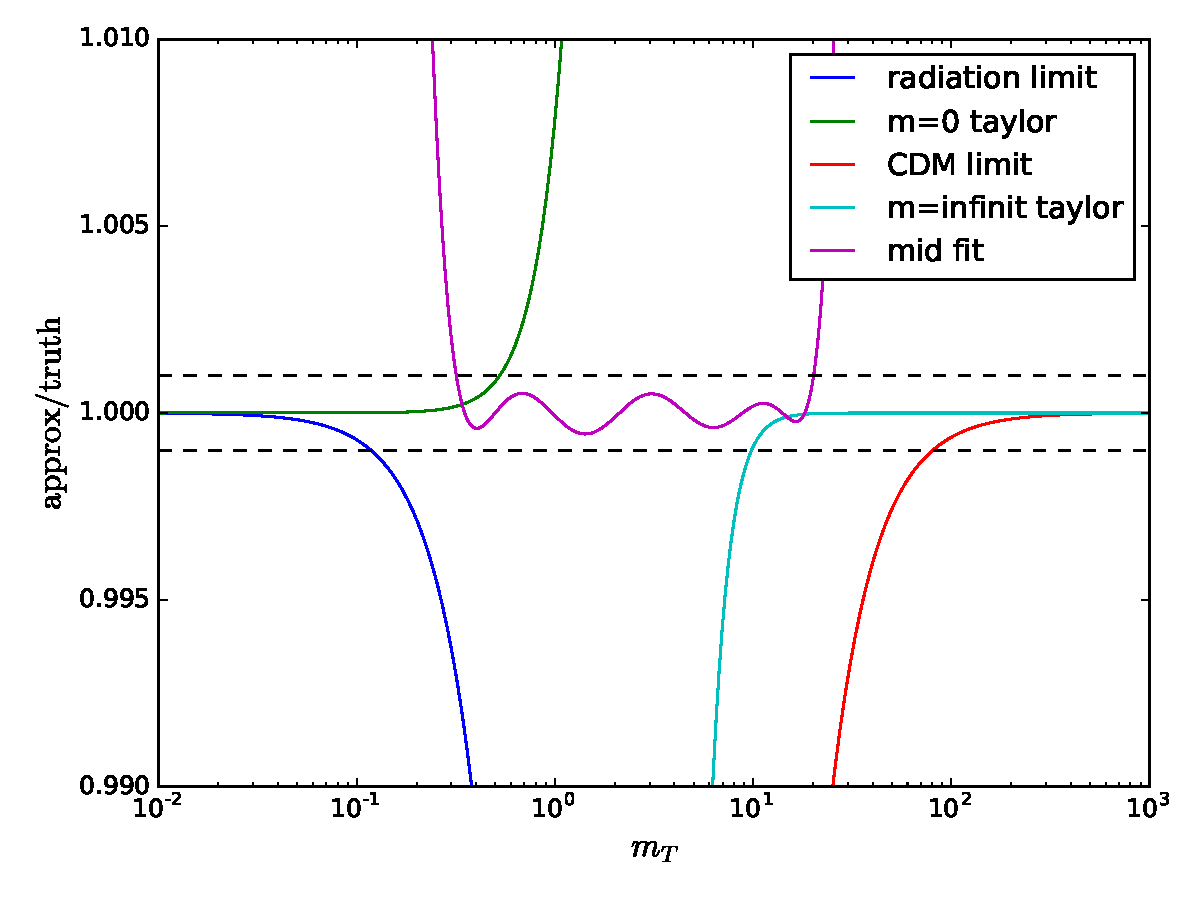
\includegraphics[width=\linewidth]{./fitfig.pdf}
  \caption{Approximations in three different regimes considered
    here. Accuracy is better than $10^{-3}$ everywhere (dashed lines).}
  \label{fig:approx}
\end{figure}


\end{document}
